\itemhead{p.76 练习 · 第3题（教材p.76）}{XJ-B1-C03-PR-P076-Y0567}
\label{XJ-B1-C03-PR-P076-Y0567}
{\footnotesize 湘教版教材p.76 / PDF第83页 / p.76 练习 / 第3题}
\field{原题}{一个质点沿直线运动。质点由静止匀加速 $T\,\mathrm s$ 后速度达到 $8\,\mathrm{m/s}$，然后质点以恒定速度 $8\,\mathrm{m/s}$ 运动了 $5T\,\mathrm s$，之后质点在 $40\,\mathrm s$ 内匀减速到完全停下。
\subq{1}画出质点运动的速度-时间图象；
\subq{2}已知质点运动的总位移是 $600\,\mathrm m$，求 $T$ 的值；
\subq{3}画出质点运动的加速度-时间图象。}
\field{参考答案}{（1）$v(t)=8t/T$（$0\le t\le T$）、8（$T<t\le6T$）、$8-(t-6T)/5$（$6T<t\le6T+40$）；折线经过 $(0,0),(T,8),(6T,8),(6T+40,0)$。（2）面积给出 $44T+160=600$，故 $T=10$ s。（3）在三个运动阶段内部 $a=0.8,0,-0.2$（米每二次方秒）；理想模型在速度折点处不要求加速度存在。}
\begin{center}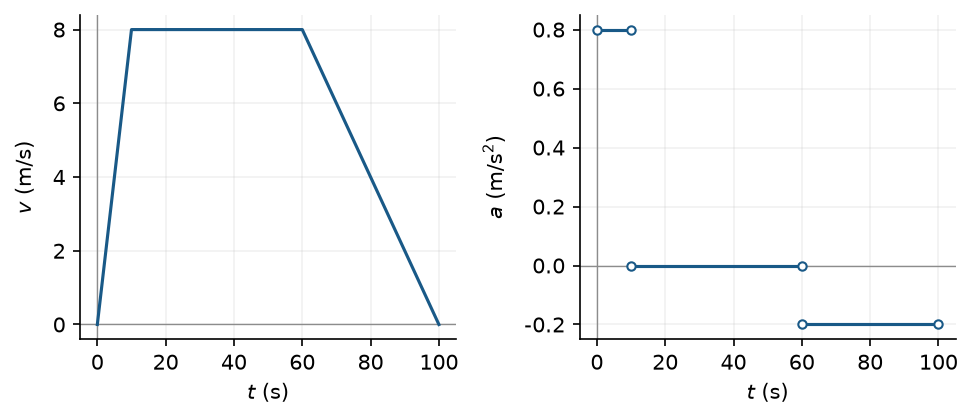
\includegraphics[width=.84\linewidth,height=.38\textheight,keepaspectratio]{figures/C03-PR076-3.png}\end{center}
{\small \field{关联知识}{F07 分段函数、绝对值及分段应用（教材帮p.86、91、92、93 / PDF95、100、101、102）；F04 函数三种表示法、图象与读数（教材帮p.85、86、93、94 / PDF94、95、102、103）}
\field{方法与易错点}{先列转折点和各段条件，再建立分段式，检查衔接、定义域与值域。 易错：跨段套公式；超额部分按全量收费；绝对值去号漏区间。}
\field{答案依据}{答案册相关题组：PDF第20页（册内页19）；按当前题库原题逐项重算，不按旧版题号机械对套。}}
